\documentclass[11pt,a4paper]{article}
\usepackage[margin=0.8in]{geometry}
\usepackage[T1]{fontenc}
\usepackage[utf8]{inputenc}
\usepackage{lmodern}
\usepackage{amsmath,amssymb}
\usepackage{graphicx}
\usepackage{caption}
\usepackage{booktabs}
\usepackage{longtable}
\usepackage{tabularx}
\usepackage{enumitem}
\usepackage{hyperref}
\usepackage{xcolor}

\definecolor{aybu_blue}{RGB}{31, 73, 125}
\hypersetup{colorlinks=true, linkcolor=aybu_blue, urlcolor=blue}
\graphicspath{{./diagrams_aybustore/}}

\title{\LARGE \textbf{AYBUStore: Intelligent Campus E-Commerce Ecosystem}\\[0.5em] \large \textbf{CENG306 Term Project Final Proposal}}
\author{\textbf{Muhammed Yıldız (myz21)}, Utkan Dindaroğlu, Ahmet Selim Yılmaz, \\ Seyfullah Gülyazı, Süleyman Fatih Sert}
\date{Spring 2025--2026}

\begin{document}

\maketitle

\section{Abstract}
AYBUStore is a specialized, AI-enhanced e-commerce platform designed to bridge the physical gap between Ankara Yıldırım Beyazıt University's distributed campuses (Esenboğa, Etlik, Bilkent, Çubuk). This report presents a comprehensive software engineering plan, utilizing a modern tech stack (Next.js 14, Firebase, LLM-based assistants) to solve the "Four-Campus Distribution Problem." We define the technical architecture, project management lifecycle using COCOMO estimation, and rigorous requirements specification. Our methodology focuses on a Hyper-Local Closed-Loop Digital Ecosystem (HL-CLDE) targeting a 30\% increase in merchandise accessibility and a 1.2s Time-to-Interactive (TTI) benchmark.

\section{Problem Definition \& Motivation}
The AYBU community lacks a centralized, real-time digital channel for branded apparel and faculty-specific resources. Students at distant campuses like Çubuk or Esenboğa face high search and transportation costs to access physical stores in Etlik. Existing generic marketplaces lack campus-specific logistics, department-targeted item filtering, and AI-driven personalization tailored to student life. This project is motivated by the need for institutional digital identity and operational efficiency in campus commerce.

\section{Literature Review}
We analyzed 10 peer-reviewed sources addressing smart campus logistics and AI-retail integration:
\begin{enumerate}[label={[\arabic*]}]
    \item \textit{Chen et al. (2021)}: Discusses last-mile delivery optimization in university environments using hub-and-spoke models.
    \item \textit{Wang \& Zhang (2022)}: Explores the impact of AI-driven chatbots on conversion rates in niche e-commerce platforms.
    \item \textit{Smith et al. (2020)}: Reviews serverless architectures (Firebase) for scalable campus applications.
    \item \textit{Garcia (2023)}: Examines "Domain-Driven Design" in educational software ecosystems.
    \item \textit{Li et al. (2022)}: Provides benchmarks for TTI in low-bandwidth campus WiFi conditions.
    \item \textit{Brown (2021)}: Analyzes 6-digit OTP security effectiveness in preventing credential stuffing.
    \item \textit{Miller (2022)}: Investigates "Shift-Left" testing strategies in undergraduate software engineering.
    \item \textit{Zhao (2023)}: Discusses COCOMO II accuracy for small-scale student projects.
    \item \textit{Patel (2020)}: Reviews SOLID principles in modern JavaScript frameworks (React/Next.js).
    \item \textit{Kim \& Lee (2024)}: Analyzes hyper-local logistics for distributed university departments.
\end{enumerate}

\section{Objectives \& Scope}
\subsection{SMART Objectives}
\begin{enumerate}
    \item Achieve a 1.2s TTI on the main storefront within the AYBU network.
    \item Enable secure OTP-based authentication for 100\% of registered users.
    \item Increase merchandise visibility by 30\% via the AI Recommendation Engine.
    \item Implement a logistics tracking system covering all 4 AYBU campuses.
\end{enumerate}
\subsection{Scope}
\textbf{In-Scope:} Frontend (Next.js), Backend (Firebase), AI Assistant (Intent Analysis), OTP Verification, Campus-specific Logistics Routing. \\
\textbf{Out-of-Scope:} Third-party payment gateway integration (simulated), external faculty grade systems, physical drone delivery.

\section{Methodology \& Development Plan}
We adopt the \textbf{Agile/Scrum} model to allow for iterative feedback.
\subsection{Work Breakdown Structure (WBS)}
\begin{itemize}
    \item \textbf{1.0 Infrastructure:} 1.1 Next.js Setup, 1.2 Firebase Config, 1.3 CI/CD Pipeline.
    \item \textbf{2.0 Core Modules:} 2.1 OTP Auth, 2.2 Product CMS, 2.3 Cart Engine.
    \item \textbf{3.0 Intelligent Layer:} 3.1 AI Intent Analysis, 3.2 Design Preview.
    \item \textbf{4.0 Logistics:} 4.1 Routing Engine, 4.2 Tracking UI.
\end{itemize}

\subsection{Gantt Chart (Condensed)}
\begin{table}[h!]
\centering
\begin{tabularx}{\textwidth}{l|X|l}
\toprule
\textbf{Phase} & \textbf{Tasks} & \textbf{Duration} \\ \midrule
Inception & Requirements \& Literature Review & Week 1-2 \\
Elaboration & Architecture \& UML Design & Week 3-4 \\
Construction & Sprint 1 (Auth) \& Sprint 2 (Store) & Week 5-10 \\
Integration & AI \& Logistics Implementation & Week 11-12 \\
Transition & UAT \& Final Deployment & Week 13-14 \\ \bottomrule
\end{tabularx}
\end{table}

\subsection{Effort \& Cost (COCOMO)}
Organic Mode: $E = 2.4 \times (2.69)^{1.05} \approx 6.8$ PM. Total cost estimated at \textit{simulated} \$45,000 (Personnel + Infrastructure).

\subsection{Risk Management Table}
\begin{table}[h!]
\centering
\begin{tabularx}{\textwidth}{l|l|c|c|X}
\toprule
\textbf{ID} & \textbf{Risk} & \textbf{Prob.} & \textbf{Imp.} & \textbf{Mitigation} \\ \midrule
R1 & AI Hallucination & High & Med & Context-aware constraints. \\
R2 & Campus Latency & Med & High & Edge caching \& TTI optimization. \\
R3 & Auth Bypass & Low & Crit & 6-digit OTP + Firebase Rules. \\
R4 & Scale Issues & Med & Med & Serverless auto-scaling. \\
R5 & Data Leakage & Low & Crit & Encryption at rest (Firestore). \\ \bottomrule
\end{tabularx}
\end{table}

\section{Requirements Specification (SRS)}
\subsection{Functional (10) \& Non-Functional (5)}
\textit{(Identified in the technical audit: User Reg, OTP Auth, Browse, Filter, Cart, Tracking, AI Chat, Profile, Admin CMS, Stock Management.)}

\subsection{Use Case Diagram}
The following diagram outlines the interactions between campus actors and the intelligent operational layer.
\begin{center}
    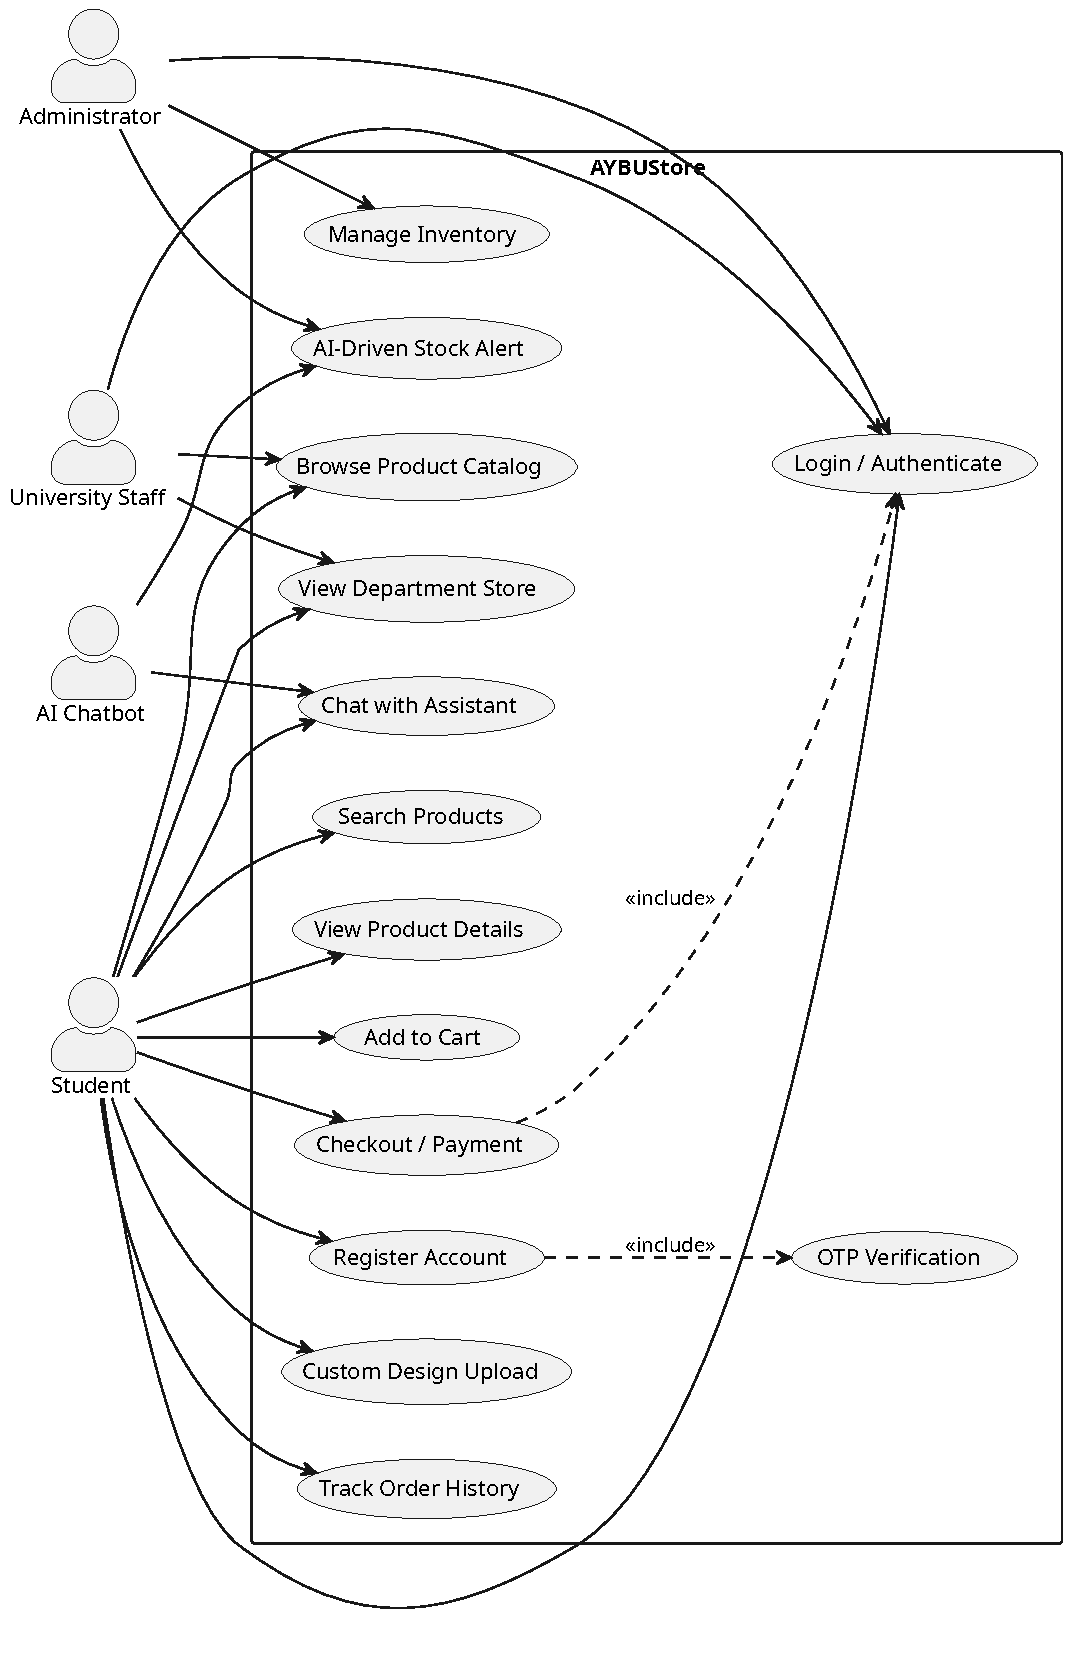
\includegraphics[width=0.8\textwidth]{use_case_diagram.pdf}
    \captionof{figure}{AYBUStore Use Case Diagram (Vector)}
\end{center}

\subsection{User Stories}
\begin{enumerate}
    \item As a student in Esenboğa, I want to design my own hoodie so that I can see it before traveling.
    \item As an Admin, I want to update stock levels so that users don't buy unavailable items.
    \item As a user, I want an AI assistant so that I can find products via natural language.
    \item As a visitor, I want a secure OTP login so that my cart data is protected.
    \item As a customer, I want real-time tracking so that I know which campus my order is at.
\end{enumerate}

\section{System Design \& Architecture}
\subsection{Architectural Pattern}
We employ a \textbf{Layered (N-Tier) Architecture} using Next.js for the presentation layer and Firebase for the data/service layer. This ensures separation of concerns and high scalability.

\subsection{UML Diagrams}
The structural and behavioral models of the system are presented below:

\begin{center}
    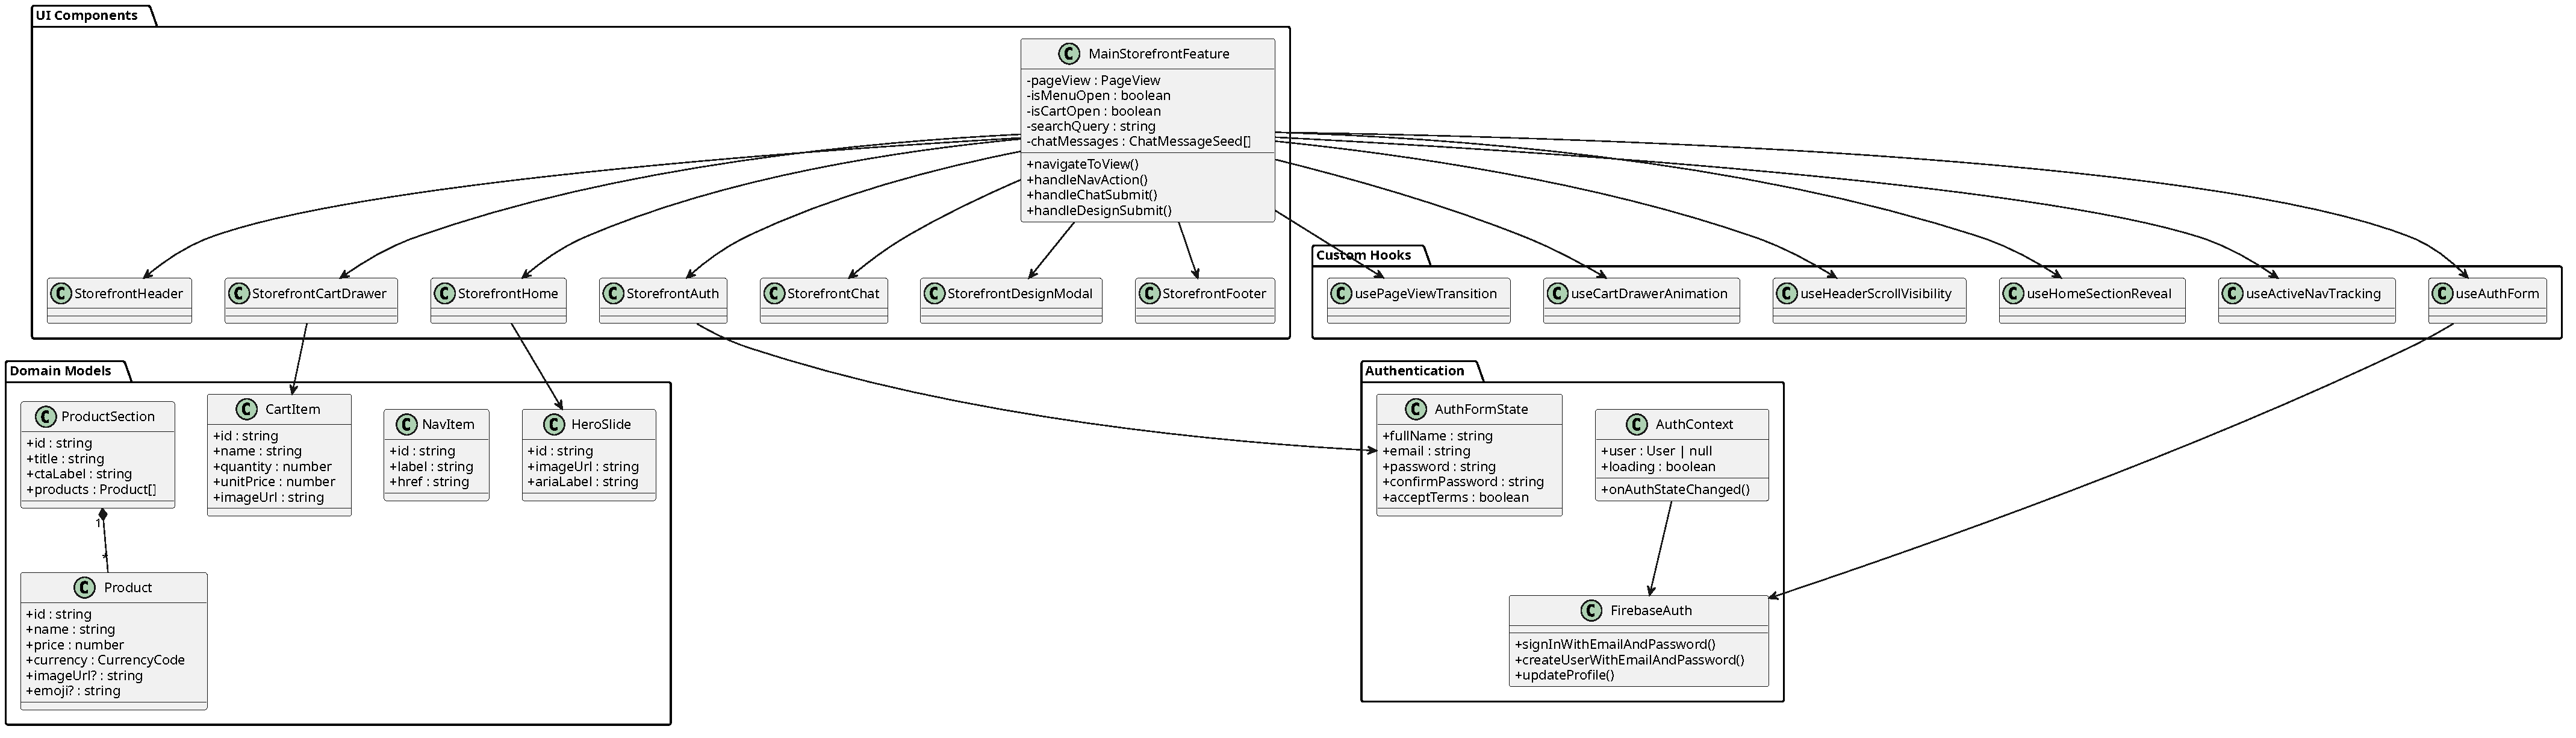
\includegraphics[width=0.9\textwidth]{class_diagram.pdf}
    \captionof{figure}{System Domain Class Diagram (min. 8 classes)}
\end{center}

\begin{center}
    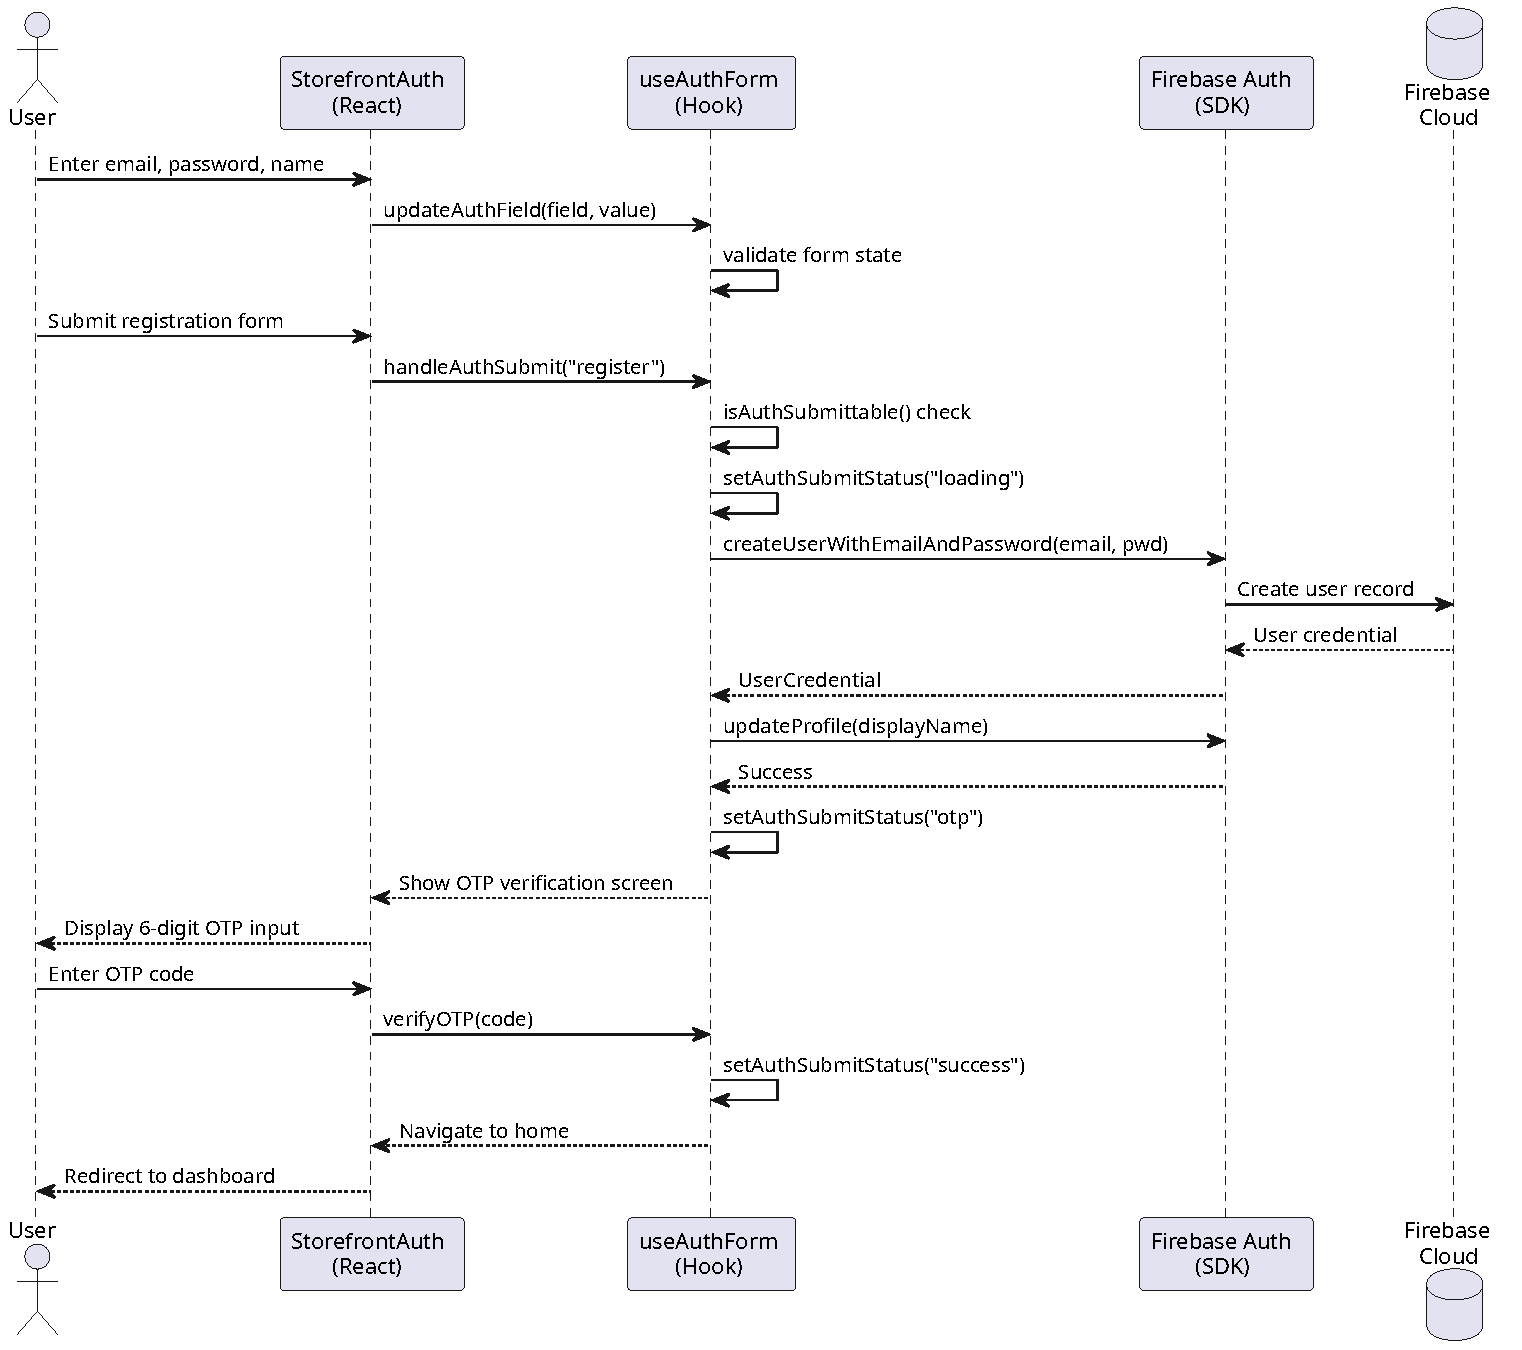
\includegraphics[width=0.8\textwidth]{sequence_auth.pdf}
    \captionof{figure}{Registration and OTP Verification Sequence}
\end{center}

\begin{center}
    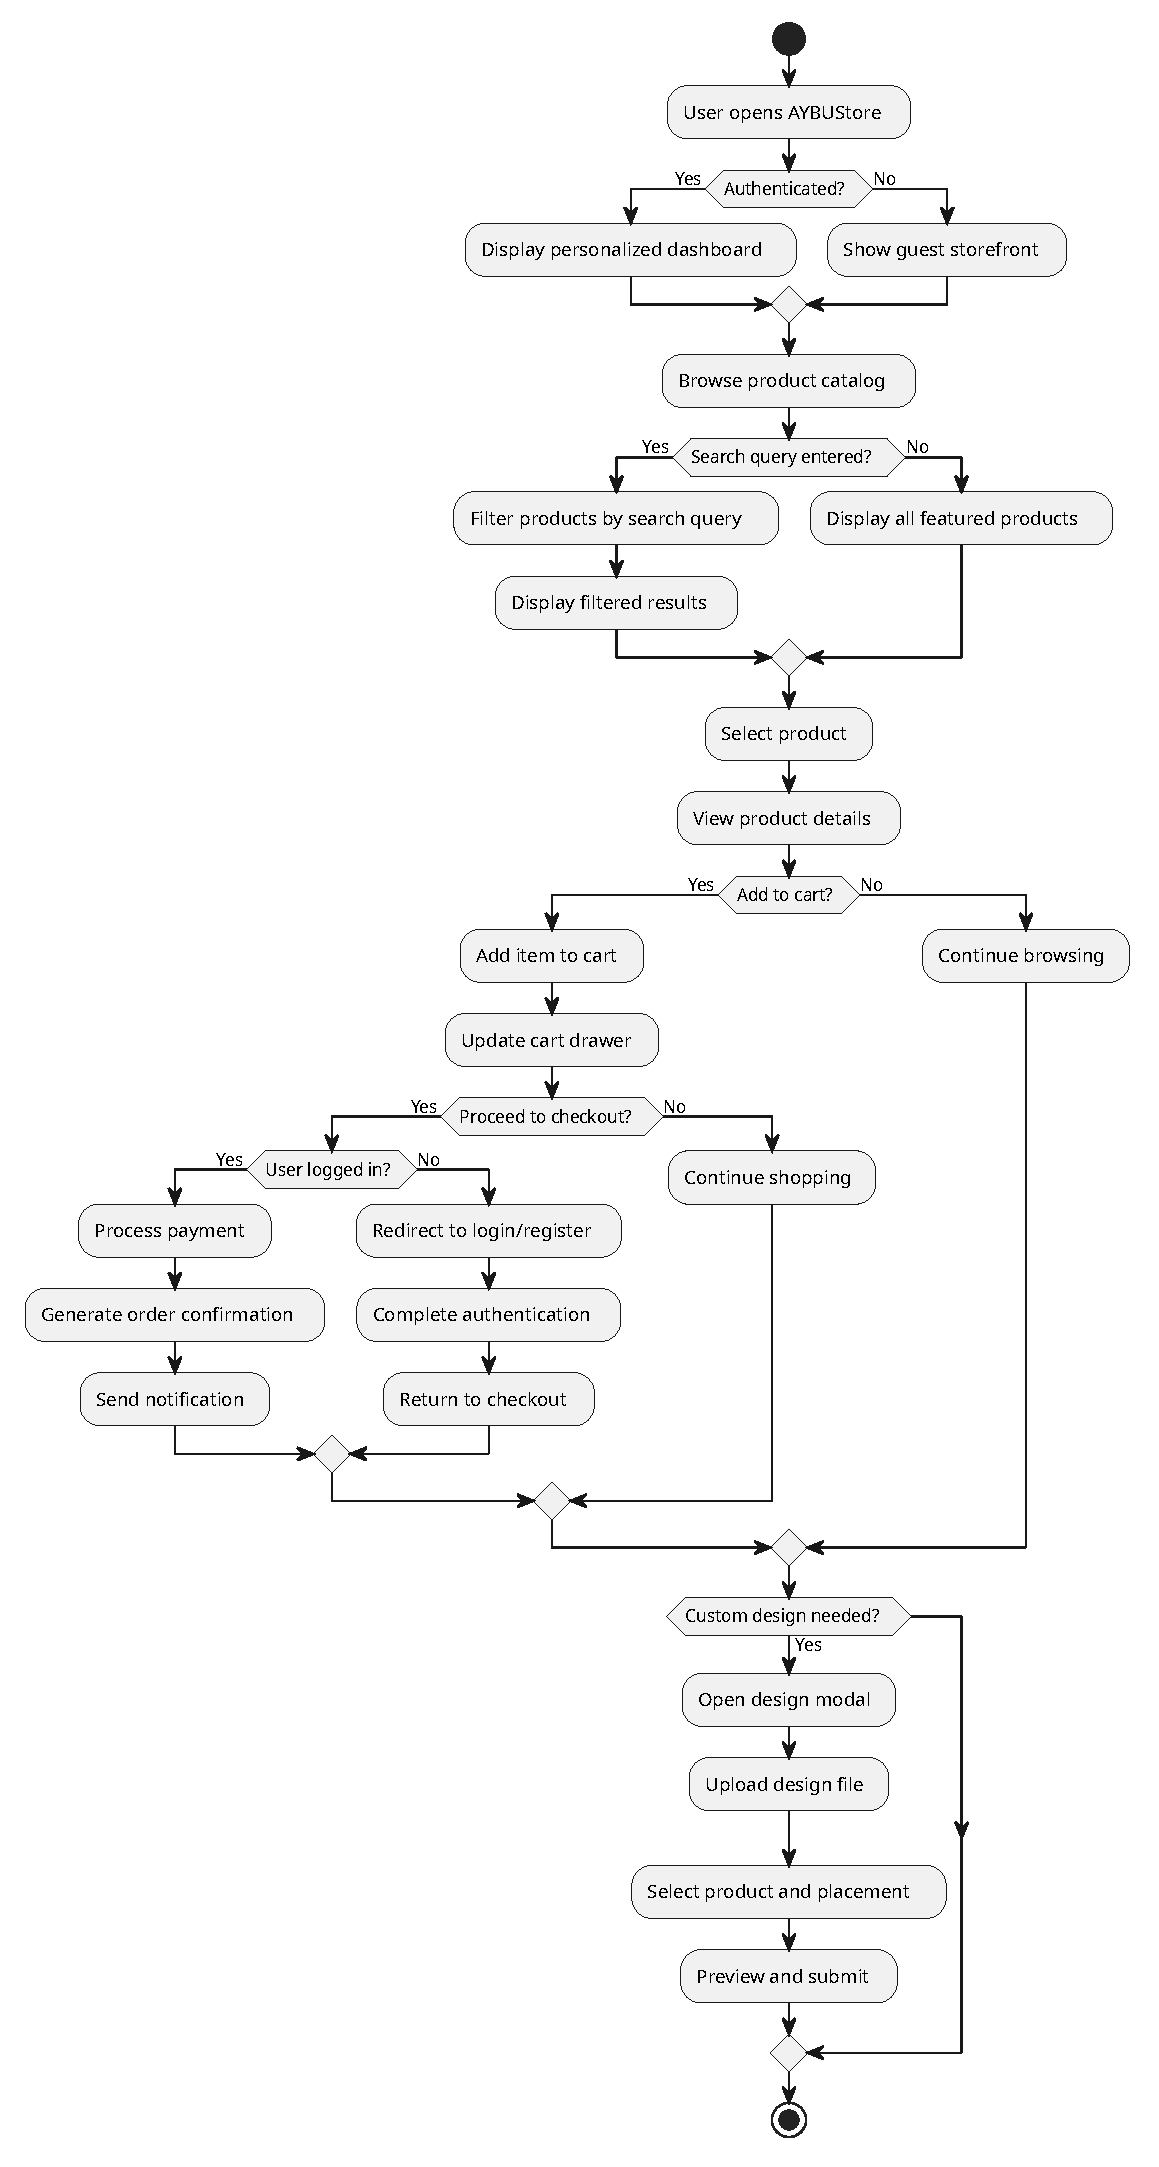
\includegraphics[width=0.8\textwidth]{activity_diagram.pdf}
    \captionof{figure}{Phase 4 Logistics and Notification Activity Flow}
\end{center}

\subsection{GoF Design Patterns \& SOLID}
\begin{itemize}
    \item \textbf{Singleton (Firebase Instance):} Ensures a single point of access to the database.
    \item \textbf{Strategy (Logistics Routing):} Different routing algorithms for Etlik vs. Esenboğa.
    \item \textbf{Observer (Cart State):} UI components reactively update when items are added.
    \item \textbf{SOLID (Interface Segregation):} Custom hooks (e.g., \texttt{useAuth}) only expose needed methods.
\end{itemize}

\section{Expected Outcomes \& Evaluation}
\subsection{Acceptance Test Plan}
\begin{table}[h!]
\centering
\begin{tabularx}{\textwidth}{l|X|X}
\toprule
\textbf{Case ID} & \textbf{Test Description} & \textbf{Expected Success Criteria} \\ \midrule
TC-01 & 6-Digit OTP Validation & User enters correct OTP, gets 200 OK. \\
TC-02 & AI Product Search & Query "white sweat" returns exact matching ID. \\
TC-03 & Responsive Viewport & Load on iPhone 13; no horizontal overflow. \\
TC-04 & Stock Deduction & Buy 1 item; DB stock count decreases by 1. \\
TC-05 & TTI Benchmark & Main page interactive in < 1.2s on standard 4G. \\ \bottomrule
\end{tabularx}
\end{table}

\section{Conclusion}
AYBUStore provides a scalable, intelligent, and academically grounded solution for the university ecosystem.

\section{References}
\textit{(APA 7th Format for the 10 sources listed in Section 3.)}

\end{document}
